\documentclass[11pt,a4paper]{scrartcl}
\typearea{12}
\usepackage{graphicx}
\usepackage{pstricks}
\usepackage{listings}
\pagestyle{headings}
\markright{Draw a Neuron}
\begin{document}

\section*{Draw a Neuron\footnote{\texttt{github.com/conorhoughton/teaching\_misc/tree/master/python\_workshop}}}

This is a picture drawn by Santiago Ram\'{o}n y Cajal of cells in the human forebrain:
\begin{center}
\includegraphics{images/cajal.png}
\end{center} 
It shows two different cell types, A-E are pyramidal cells, F and K are interneurons. These links bring you to some more pictures 
\begin{itemize}
\item \texttt{ecee.colorado.edu/~ecen4831/cnsweb/cns2a.html}
\item \texttt{www.nature.com/nrn/journal/v9/n3/fig\_tab/nrn2286\_F1.html}
\item \texttt{http://bit.ly/1T7TB0x}
\end{itemize}
It is intesteresting to consider how these shapes are formed and
informative to try writing a programme to draw them. In the
\texttt{draw\_a\_neuron} folder in the github you can see my attempt,
it makes neurons that look like this:
\begin{center}
\fbox{
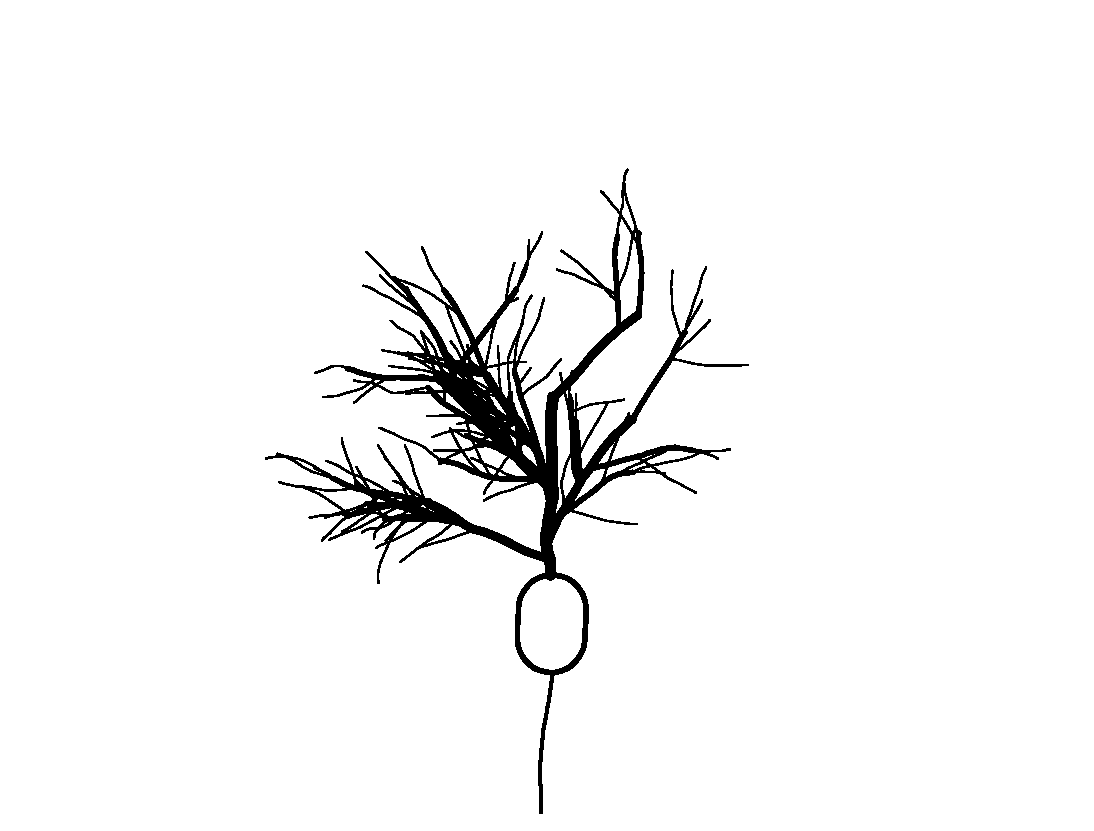
\includegraphics[width=10cm]{eps/neuron.eps}}
\end{center}
Probably you can do better, have a go; either by modifying my
programme or writing your own.
\end{document}
